\documentclass[twocolumn]{article}
\usepackage{sty/simple}
\usepackage{graphicx} % Required for inserting images
\usepackage[maxbibnames=99]{biblatex}
\usepackage{cuted}
\addbibresource{6.7900.bib} 

% \documentclass[a4paper]{article}
% \usepackage[a4paper, portrait, margin=1in]{geometry}

% other stuff
\usepackage{import}
\subimport{sty}{init}
\usetikzlibrary{positioning}
\usetikzlibrary{3d} %for including external image 
\subimport{sty}{diagramimports}

\usepackage{multicol}

\title{{\LARGE 6.7900 Final Project: Exploring Artwork Style-Content Interaction in Image Classification Models}}
\author{Katie Chen and Andrew Liu}
\date{December 15, 2023}

\begin{document}

\maketitle

\begin{abstract}

In this project, we study the problem of classifying artwork by \textit{style} using artistic images in the ArtBench dataset \cite{liaoArtBenchDatasetBenchmarking2022a}. We find that deep convolutional neural networks (CNNs) like ResNet50 \cite{heDeepResidualLearning2015} and VGG19 \cite{simonyanVeryDeepConvolutional2014} are much better suited to learning artwork style than diffusion-based classifier models, where ResNet50 achieves $97\%$ classification accuracy on a binary classification task, VGG19 achieves $99\%$, and a diffusion-based model achieves $81\%$. We further investigate the success of VGG19 in its classification task with a series of manual feature extraction tasks. In particular, by training linear probes with features extracted at different layers in the network, and introducing visual heuristics with Principal Component Analysis (PCA), we find that the depth of VGG19 plays a key role in its success classifying artwork. The models' ability to confidently express style-related learning almost directly correlates with model depth, ultimately suggesting that \textit{style} in artwork is a layered visual characteristic. 

\end{abstract}

\section{Introduction}
% The burgeoning field of artwork classification via neural networks has gained significant traction, propelled by advancements in deep learning. The interplay between style and content in artwork has emerged as a subject of significant interest and challenge. We aim to understand how contemporary image classification models perceive and process the stylistic and content-driven aspects of artwork. 
The field of artwork classification via neural networks has gained significant traction propelled by advancements in deep learning. The interplay between \textit{style} and \textit{content} in artwork has emerged as a subject of significant interest and challenge. We are interested in exploring which modern architectures are best suited to learn image \textit{style}, and how architectures which are effective are able to perceive and process the style-content interaction in artwork. The first notions of style-content interaction in image classification were introduced by Gatys et al. \cite{gatysNeuralAlgorithmArtistic2015}, in their paper introducing the Neural Style Transfer algorithm.

% \textit{Style}, as defined by Gatys et al. in their seminal work on neural style transfer, is the ``texturised versions of the input image that capture its general appearance in terms of colour and localised structures'' \cite{gatysNeuralAlgorithmArtistic2015}. Content refers to the discernible objects and figures depicted within the artwork. It encompasses the subject matter and the representational elements that are portrayed, independent of the artistic style. In the context of image classification models, content can be understood as the arrangement of different high-level features such as shapes and structures that come together to form the recognizable entities within an image. These elements are what enable viewers to interpret and derive meaning from the artwork, identifying what is depicted rather than how it is stylistically presented. 
\textit{Style}, as defined by Gatys et al., is the ``texturised versions of the input image that capture its general appearance in terms of colour and localised structures'' \cite{gatysNeuralAlgorithmArtistic2015}. \textit{Content} refers to the discernible objects and figures depicted within the artwork, independent of artistic style. Artwork analysis is particularly complex because nuances in style and content make learning artistic images not just a matter of recognizing pixel-based patterns, as is the case for most image classification tasks; instead, there are also intangible and subjective elements at play.

% We recognize the unique complexities inherent in artwork analysis, which differ substantially from conventional image processing tasks. Artistic images are not merely repositories of pixel-based information but are imbued with layers of historical, cultural, and subjective elements that are often encapsulated in the style and content of the artwork. This duality poses a distinct challenge for automated image classification systems, which typically excel at recognizing overt, tangible features but may struggle to interpret the nuanced interplay of style and content. 

In our project, we first compare how deep CNN architectures, particularly ResNet50 and VGG19, compare to diffusion model classifiers in the style classification task. We fine-tune these deep CNNs on the ArtBench dataset \cite{liaoArtBenchDatasetBenchmarking2022a}, and implement the diffusion classifier in \cite{liYourDiffusionModel}. After showing that neural net architectures are more effective, we then further investigate how they are able to break down the style-content representation of artwork effectively through feature extraction of the networks. We select five different layers in the network to extract features from and train linear probing classifiers to study the evolution of how the network perceives the image. We also visualize this evolution by employing PCA on the extracted features. Ultimately, we find that deeper layers in the network capture predominantly style-related information to more content-specific details, suggesting a layered understanding to the visual characteristics that define an artwork.

% In our project, we study how deep convolutional neural networks (CNNs), specifically the VGG19 model, differentiate and learn from the stylistic and content-related aspects of artwork. By extracting features from various layers of the CNN, training linear probing classifiers, and employing dimensionality reduction techniques such as Principal Component Analysis (PCA), we observe how the network's perception evolves across different levels of abstraction. Our findings reveal that as we progress through the layers of the network, the extracted features transition from capturing predominantly style-related information to more content-specific details, suggesting a layered understanding of the visual characteristics that define an artwork. 


\section{Related Works}

A notable contribution in this domain is the work by Gatys et al. (2016) \cite{gatysNeuralAlgorithmArtistic2015}, which elegantly demonstrated how CNNs can separate and recombine the content and style of natural images, laying the groundwork for automated artistic style transfer. Work like Elgammal et al. \cite{Elgammal} then furthered the narrative by applying deep learning to classify artworks into historical periods, leveraging the nuanced feature extraction capabilities of CNNs to discern artistic styles. 

% These endeavors underscored the potential of machine learning in automating the classification of art epochs and styles, thereby contributing significantly to the intersection of computational technology and art history.

% A notable contribution in this domain is the work by Gatys et al. (2016) \cite{gatysNeuralAlgorithmArtistic2015}, which elegantly demonstrated how CNNs can separate and recombine the content and style of natural images, laying the groundwork for automated artistic style transfer. This pioneering study not only enhanced the understanding of neural representations of artworks but also spurred a series of explorations into the interpretability of neural networks in art. Following this, researchers like Elgammal et al. \cite{} furthered the narrative by applying deep learning to classify artworks into historical periods, leveraging the nuanced feature extraction capabilities of CNNs to discern artistic styles. These endeavors underscored the potential of machine learning in automating the classification of art epochs and styles, thereby contributing significantly to the intersection of computational technology and art history.

% The exploration of style and content interaction in artworks using neural networks has opened new avenues in understanding the interpretability of these models. Zeiler and Fergus \cite{zeilerVisualizingUnderstandingConvolutional2013} made early strides by visualizing the intermediate layers of CNNs, providing insights into the hierarchical feature learning process. This methodology shed light on how neural networks perceive artistic content and style, serving as a precursor to more sophisticated interpretability frameworks. More recent studies, such as those by Bau et al. \cite{bauNetworkDissectionQuantifying2017}, have delved deeper into disentangling and interpreting the layers of neural networks, particularly in the context of generative models. 

The exploration of style and content interaction in artworks using neural networks has opened new avenues in understanding the interpretability of these models. Zeiler and Fergus \cite{zeilerVisualizingUnderstandingConvolutional2013} made early strides by visualizing the intermediate layers of CNNs, providing insights into the hierarchical feature learning process. This methodology shed light on how neural networks perceive artistic content and style. Studies such as those by Bau et al. \cite{bauNetworkDissectionQuantifying2017} have delved deeper into interpreting the layers of neural networks, particularly in the context of generative models. 

% the strip here is necessary because tikz won't behave in a figure*. idk why
\begin{strip}
\begin{figure}[H]
\scalebox{0.5}{%
\begin{tikzpicture}
\tikzstyle{connection}=[ultra thick,every node/.style={sloped,allow upside down},draw=\edgecolor,opacity=0.7]

%%%%%%%%%%%%%%%%%%%%%%%%%%%%%%%%%%%%%%%%%%%%%%%%%%%%%%%%%%%%%%%%%%%%%%%%%%%%%%%%%%%%%%%%
%% Draw Layer Blocks
%%%%%%%%%%%%%%%%%%%%%%%%%%%%%%%%%%%%%%%%%%%%%%%%%%%%%%%%%%%%%%%%%%%%%%%%%%%%%%%%%%%%%%%%
% input
\pic[shift={(0,0,0)}] at (0,0,0) {
    Box={
            name=input,
            caption=Input,
            xlabel= 3,
            ylabel=224,
            zlabel= \qquad 224,
            fill=\ConvColor,
            height=40,
            width=0.1,
            depth=40
        }
};
% conv1_1,conv1_2
\pic[shift={(0,0,0)}] at (2.5,0,0) {
RightBandedBox={
name=cr1,
caption=conv1,
xlabel={{"64","64"}},
zlabel=224,
fill=\ConvColor,
bandfill=\ConvReluColor,
height=40,
width={2,2},
depth=40
}
};
%pool1
\pic[shift={(0,0,0)}] at (cr1-east) {
Box={
name=p1,
fill=\PoolColor,
opacity=0.5,
height=35,
width=1,
depth=35
}
};
%%%%%%%%%%
% conv2_1,conv2_2
\pic[shift={(2,0,0)}] at (p1-east) {
RightBandedBox={
name=cr2,
caption=conv2,
xlabel={{"128","128"}},
zlabel=112,
fill=\ConvColor,
bandfill=\ConvReluColor,
height=35,
width={3,3},
depth=35}
};
%pool2
\pic[shift={(0,0,0)}] at (cr2-east) {
Box={
name=p2,
fill=\PoolColor,
opacity=0.5,
height=30,
width=1,
depth=30}
};
%%%%%%%%%%
% conv3_1,conv3_2,conv3_3,conv3_4
\pic[shift={(2,0,0)}] at (p2-east) {
RightBandedBox={
name=cr3,
caption=conv3,
xlabel={{"256","256","256","256"}},
zlabel=56,
fill=\ConvColor,
bandfill=\ConvReluColor,
height=30,
width={4,4,4,4},
depth=30}
};
%pool3
\pic[shift={(0,0,0)}] at (cr3-east) {
Box={
name=p3,
fill=\PoolColor,
opacity=0.5,
height=23,
width=1,
depth=23}
};
%%%%%%%%%%
% conv4_1,conv4_2,conv4_3,conv4_4
\pic[shift={(1.8,0,0)}] at (p3-east) {
RightBandedBox={
name=cr4,
caption=conv4,
xlabel={{"512","512","512","512"}},
zlabel=28,
fill=\ConvColor,
bandfill=\ConvReluColor,
height=23,
width={7,7,7,7},
depth=23}
};
%pool4
\pic[shift={(0,0,0)}] at (cr4-east) {
Box={
name=p4,
fill=\PoolColor,
opacity=0.5,
height=15,
width=1,
depth=15}
};
%%%%%%%%%%
% conv5_1,conv5_2,conv5_3,conv5_4
\pic[shift={(1.5,0,0)}] at (p4-east) {
RightBandedBox={
name=cr5,
caption=conv5,
xlabel={{"512","512","512","512"}},
zlabel=14,
fill=\ConvColor,
bandfill=\ConvReluColor,
height=15,
width={7,7,7,7},
depth=15}
};
%pool5
\pic[shift={(0,0,0)}] at (cr5-east) {
Box={
name=p5,
fill=\PoolColor,
opacity=0.5,
height=10,
width=1,
depth=10}
};
%%%%%%%%%     
% fullconnection
\pic[shift={(2.5,0,0)}] at (p5-east) {
    RightBandedBox={
            name=cr6,
            caption=\makebox[0pt]{\shortstack[c]{fc}},
            xlabel={{"",""}},
            zlabel=25088,
            fill=\FcColor,
            bandfill=\SoftmaxColor,
            height=2,
            width=2,
            depth=70
        }
};
%%%%%%%%%%%%%%%%%%%%%%%%%%%%%%%%%%%%%%%%%%%%%%%%%%%%%%%%%%%%%%%%%%%%%%%%%%%%%%%%%%%%%%%
% Draw connections
%%%%%%%%%%%%%%%%%%%%%%%%%%%%%%%%%%%%%%%%%%%%%%%%%%%%%%%%%%%%%%%%%%%%%%%%%%%%%%%%%%%%%%%
\draw [connection]  (0,0,0)    -- node {\midarrow} (cr1-west);
\draw [connection]  (p1-east)    -- node {\midarrow} (cr2-west);
\draw [connection]  (p2-east)    -- node {\midarrow} (cr3-west);
\draw [connection]  (p3-east)    -- node {\midarrow} (cr4-west);
\draw [connection]  (p4-east)    -- node {\midarrow} (cr5-west);
\draw [connection]  (p5-east)    -- node {\midarrow} (cr6-west);
%%%%%%%%%%%%%%%%%%%%%%%%%%%%%%%%%%%%%%%%%%%%%%%%%%%%%%%%%%%%%%%%%%%%%%%%%%%%%%%%%%%%%%%%
\end{tikzpicture}
}
\end{figure}
\vspace{-1.25cm}
\label{fig:VGG19}
Figure 2: VGG19 architecture. We fine-tuned pre-trained weights with ArtBench \cite{liaoArtBenchDatasetBenchmarking2022a}, where the final connected layer is modified to a binary classifier, or multiclass classifier. We trained linear probes on the features at the output of the five max pooling layers (dark orange) directly following each convolutional block: \verb|conv1|, \verb|conv2|, \verb|conv3|, \verb|conv4|, and \verb|conv5|. In total, this network has 140M parameters.
\end{strip}

The goal of our project is to combine the methods established by these works to produce similar results on a dataset that, unlike most other datasets, is specifically separated by style, rather than content. 
% These studies aim to unravel how different layers and neurons contribute to the overall perception of style and content in artworks, paving the way for more transparent and interpretable AI systems in the realm of art analysis. 

\section{Methodology}

\subsection{Dataset}
We use ArtBench-10, first introduced by Liao et al \cite{liaoArtBenchDatasetBenchmarking2022a}. It is the first class-balanced, high quality, cleanly annotated and standardized dataset for benchmarking artwork generation. It inlcudes 60,000 images, segmented into 10 artistic styles: \verb|art_nouveau|, \verb|baroque|, \verb|expressionism|, \verb|impressionism|, \verb|post_impressionism|, \verb|realism|, \verb|renaissance|, \verb|romanticism|, \verb|surrealism|, \verb|ukiyo_e|. Each style has 5,000 training images and 1,000 testing images. Crucially, because this dataset is purely stratified by style, we make the assumption that content is distributed uniformly across all style classes. We justify this with the advantages that the Artbench dataset asserts over previous artwork datasets, which is that it maintains class-balance and a high-quality image and annotation regime \cite{liaoArtBenchDatasetBenchmarking2022a}. This allows us to reason about networks' ability to learn style only. 

For training, we use the $256$x$256$ resolution images, cropped to $224$x$224$ resolution, for the CNN architectures and the $32$x$32$ resolution images for the diffusion classifier. For all architectures, we employ data augmentations like horizontal and vertical flips to the training set to help reduce overfitting.

% managed to train everything without the smaller set
% We separately prepared a smaller test set (henceforth referred to as the smallset) containing 100 images per class so that we can make extracting features from intermediate layers a less memory intense process. We do this by randomly sampling 100 images from the 1000 images per class and restructure them to be compatible with Pytorch ImageFolder.  

\subsection{Models}
We consider the following models: the deep CNNs ResNet50 \cite{heDeepResidualLearning2015}, VGG19 \cite{simonyanVeryDeepConvolutional2014}, as well as the diffusion classifier architecture introduced by Li et. al \cite{liYourDiffusionModel}. ResNets incorporate skip connections to enable training of very deep networks, leading to a more layered understanding of features and better performance on complex tasks, ultimately incentivizing us to investigate whether they could represent style effectively. The VGG architecture is used in the original Neural Style Transfer algorithm \cite{gatysNeuralAlgorithmArtistic2015}; see Figure~\ref{fig:VGG19} for the exact architecture we use. 

Using a diffusion model as a classifier was a novel approach to image classification, diverging from the typical discriminative model paradigm. Since CNNs and other architectures that specialize in image recognition are typically content-based learners, we were motivated to try a novel architecture. Diffusion models as classifiers could offer an advantage in handling the variability within artistic styles. Styles like surrealism exhibit a high degree of intra-class variation, which is suitable for diffusion models' generative nature. This characteristic could be particularly beneficial in differentiating artworks that share content features but diverge stylistically.

% Diffusion models, originally designed for generative tasks, have been adapted to perform classification by reversing the diffusion 

% process \cite{liYourDiffusionModel}. This process involves starting with a sample of random noise and gradually denoising it to form a coherent image that belongs to a particular class. The hypothesis is that the denoising process can learn the data distribution in such a way that it inherently distinguishes between different classes based on both style and content. 

% Furthermore, diffusion models as classifiers could offer an advantage in handling the variability within artistic styles. Given that styles like surrealism exhibit a high degree of intra-class variation \autoref{fig:surreal_ex}, a diffusion model's generative nature allows it to potentially capture this variability within its learned distribution. This characteristic could be particularly beneficial in differentiating artworks that share content features but diverge stylistically.

\subsection{Classification Task}

For each of the CNN architectures, we modified the last fully connected layer in two ways: (1) as multiclass classifiers, to identify the style belonging to a given input image, and (2) as binary classifiers, to identify whether a given image was \verb|ukiyo_e| or \verb|surrealism|. We then fine-tuned pre-trained versions of the weights across the whole network. For the diffusion classifier, we closely followed the procedure described in \cite{liYourDiffusionModel}; more details about our exact training procedure are listed in Appendix~\ref{sec:diffusionAppendix}.

% appears at the top of the next page
\begin{table*}[ht]
    \centering
    \begin{tabular}{|c|c|c|c|c|c|c|c|c|c|c|}
    \hline
    model & \verb|art| & \verb|bar| & \verb|exp| & \verb|imp| & \verb|pos| & \verb|rea| & \verb|ren| & \verb|rom| & \verb|sur| & \verb|uki| \\
    \hline
       acc  & 0.58 & 0.70 & 0.45 & 0.37 & 0.38 & 0.36 & 0.74 & 0.46 & 0.71 & 0.96 \\
    \hline
    \end{tabular}
    \caption{VGG19 test accuracy by style}
    \label{tab:vgg19_class_accuracy}
\end{table*}

Testing accuracy results after training for the three models are listed in Table~\ref{tab:initial model results}. 

\begin{table}[H]
  \centering
  % \caption{Example Table}
  \label{tab:example}
  \begin{tabular}{|p{1.5cm}|p{1.5cm}|p{1.5cm}|p{1.5cm}|}
    \hline
     & ResNet50 & VGG19 & Diffusion \\
    \hline\hline
    binary & 0.97 & 0.98 & 0.81 \\
    \hline
    multi & 0.48 & 0.57 & 0.28 \\
    \hline
  \end{tabular}
  \caption{Fine Tuned model results (test accuracy)}
  \label{tab:initial model results}  
\end{table}

Although results from the diffusion model were promising, interpretability in the context of classification is a challenge, in part because inference for the procedure described in \cite{liYourDiffusionModel} is very slow, on the order of minutes per image. The model architecture is also much less transparent than the CNN architectures, since it does not produce any intermediate features that are directly optimized for classification; they are instead optimize for a loss metric that does not lend itself to interpretability (see Appendix~\ref{sec:diffusionAppendix} for details). It is worth noting that, when trained on MNIST, our implementation of the diffusion classifier obtained $97\%$ testing accuracy, which suggests that the diffusion classifier is capable of learning the content aspect of images well. This intuitively makes sense given that the architecture for backwards inference, the UNet, is essentially another CNN that is optimized for a different image metric. Ultimately, due to the lack of easily interpretable features, we decided not to study this architecture further. 

% Although we obtained interesting results from the diffusion model, the interpretability of diffusion models in the context of classification remains a challenge, as the process by which they discern between classes is less transparent than traditional CNNs. Unlike CNNs, where one can inspect the activations and filters at various layers, diffusion models do not offer such direct insight into their internal representations. This opacity makes it difficult to directly attribute aspects of the classification decision to either style or content. 

The ResNet50 managed to achieve better results. Despite this, there was a large gap in testing vs. training accuracy in the multiclass case; the testing accuracy was $92\%$, which suggests that the model was overfit. Our best attempt to explain this overfitting, given that VGG19 and ResNet50 are both deep neural architectures who we initially expected to behave similarly, is that the ResNet50 was overfitting on content differences in the classes and not really interpreting style correctly. This is easily reinforced by skip connections, since features closer to the original image are emphasized many times over the course of learning.

VGG19 had the best classification accuracy in both tasks. This model is well known for its transfer learning capabilities, and it intuitively makes sense why it might perform better than the other models: it has very large depth, with roughly $140$M trainable parameters compared to ResNet50s $23$M, and style is a complex trait that we expect deeper networks to be able to learn better. 

% We ultimately moved forward with the VGG19 model because of its straightforward architecture that allows for easier interpretation of how the network's layers respond to different aspects of the input data. It provides a clearer framework for visualizing and understanding the convolutional filters and feature maps. Multiple stacked smaller size kernels allows for the extraction of features at varying levels of abstraction. We will refer to the fine-tuned 10 class VGG as \verb|VGG_10_class|. We also separately fine-tuned a smaller 2 class (surrealism and ukiyo\_e) VGG, which we will refer to as \verb|VGG_2_class|. 

Thus, we further analyze the VGG19 architecture to investigate aspects of the network that makes it successful at learning style. Our decision to simplify the rest of our analysis to binary classfiication was motivated by the results in Table~\ref{tab:vgg19_class_accuracy}; the model seems to recognize \verb|surrealism| and \verb|ukiyo_e| most effectively, so for the remainder of our analysis, we only consider these styles. Henceforth, \verb|VGG_10_class| refers to the fine-tuned $10$ class VGG, and \verb|VGG_2_class| refers to the fine-tuned binary classifier.

% \begin{figure}[H]
%     \centering
%     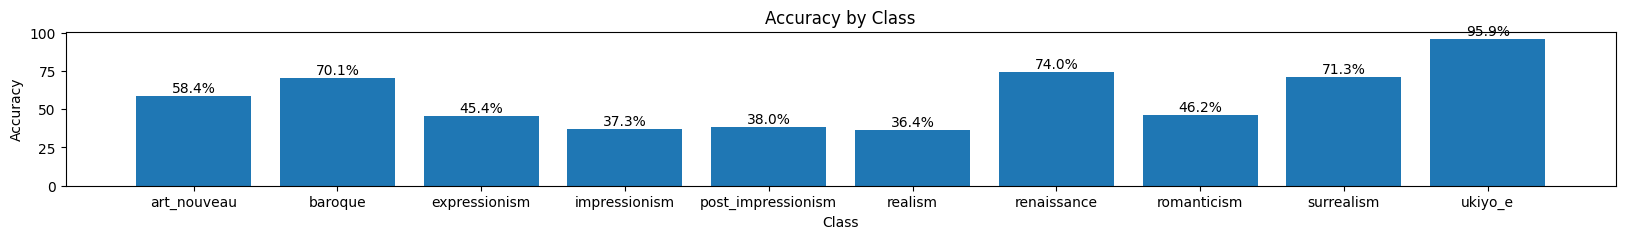
\includegraphics[width=1\linewidth]{images/retrained_vgg19_10class_accuracy.png}
%     \caption{Fine-Tuned VGG19 Classifier Accuracy by Art Style }
%     \label{fig:vgg19_class_accuracy}
% \end{figure}

\section{Results and Analysis}
\subsection{Feature Extraction}
We extracted features from \verb|conv1_1|, \verb|conv2_1|, \verb|conv3_1|, \verb|conv4_1|, \verb|conv5_1|, corresponding to the layers \verb|features.0|, \verb|features.5|, \verb|features.10|, \verb|features.19|,  \verb|features.28| from the \verb|VGG_2_class| classifier (see Figure~\ref{fig:VGG19}). We chose to analyze these layers to match the layers chosen in the paper by Gatys et al. \cite{gatysNeuralAlgorithmArtistic2015}. 

% using the smallset corresponding to the \verb|VGG_2_class| classifier. We chose these layers to extract features to match the layers chosen in the paper by Gatys et al. \cite{gatysNeuralAlgorithmArtistic2015}. 

Using these extracted features, we train a simple logistic classifier. Our results are shown in Table~\ref{tab:linear prob result}. 

\begin{table}[H]
  \centering
  \label{tab:example}
  \begin{tabular}{|l|c|c|c|c|}
    \hline
    \verb|conv1_1| & \verb|conv2_1| & \verb|conv3_1| & \verb|conv4_1| & \verb|conv5_1| \\
    \hline
    0.82 & 0.82 & 0.93 & 0.95 & 0.97 \\
    \hline
  \end{tabular}
  \caption{Linear Probing Classifier Results}
  \label{tab:linear prob result}
\end{table}

The increasing accuracy suggests that higher-level features are more effective in distinguishing between \verb|surrealism| and \verb|ukiyo_e|. Early layers like \verb|conv1_1| and \verb|conv2_1| tend to capture stylistic features like edges and textures. The deeper layers like \verb|conv5_1| are capable of capturing high-level content. The way objects are depicted in \verb|surrealism| is inherently different from \verb|ukiyo_e|, not just in color or texture but also in form and composition. This might explain why deeper layers, which capture these complex interactions, perform better in classification. Different art styles also emphasize different spatial hierarchies. \verb|ukiyo_e|, for example, has a distinct flatness and pattern-oriented approach, while surrealism often plays with perspective and depth in unconventional ways. Deeper layers of the network, which capture higher-order spatial hierarchies, are likely better at identifying these style-specific spatial characteristics.

\begin{figure*}[ht]
    \centering
    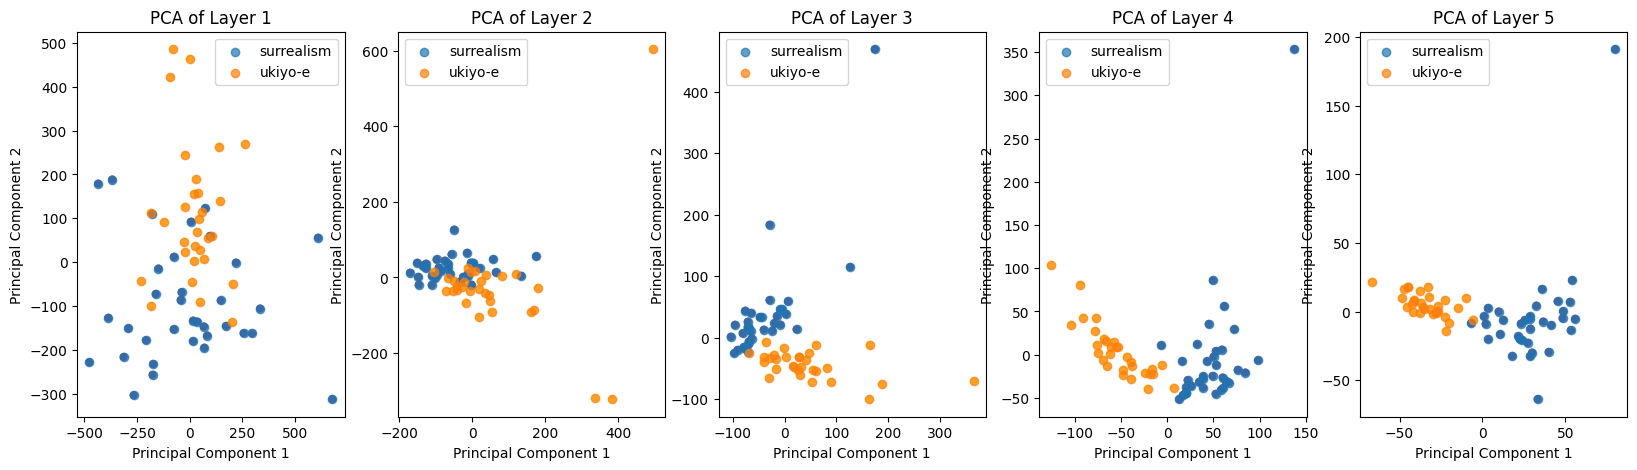
\includegraphics[width=1\linewidth]{images/pca_results.png}
    \caption{First two Principal Components from manually extracted features}
    \label{fig:pca_results}
\end{figure*}

In addition to our linear probes, we also create a visual heuristic for style understanding with PCA. For each of the five layers that we probed, we fit a PCA matrix on features extracted from the testing set; the two principal components are plotted in Figure~\ref{fig:pca_results}. The PCA results from layer \verb|conv5_1| shows the two classes almost perfectly separated along the first principal component, which suggests the extracted features provides a highly discriminative representation of the two art styles. Surrealism also apprears to be more spread out in the \verb|conv5_1|. We suspect that this is caused by the inherent style variability; surrealism is known for its broad range of styles and techniques. This diversity could result in a wider spread of feature representations even after being abstracted by the deeper layers of the network. 

% \begin{figure*}[htp]
%   \centering
%   % Only one row with two images
%   \begin{subfigure}[b]{0.49\textwidth}
%     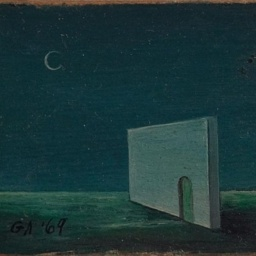
\includegraphics[width=\textwidth]{images/Abercrombie_1969_Doorway.jpg}
%     \caption{Doorway by Gertrude Abercrombie}
%   \end{subfigure}
%   \hfill
%   \begin{subfigure}[b]{0.49\textwidth}
%     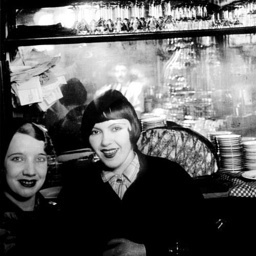
\includegraphics[width=\textwidth]{images/brassai_girls-in-paris-1932.jpg}
%     \caption{Girls in Paris by Brassai}
%   \end{subfigure}

%   \caption{Surrealism Examples}
%   \label{fig:surreal_ex}
% \end{figure*}

\subsection{Content and Style Reconstruction}
We implement the methods outlined by Gatys et. al \cite{gatysNeuralAlgorithmArtistic2015} and reconstructed style and content from \verb|conv1_1|, \verb|conv2_1|, \verb|conv3_1|, \verb|conv4_1|, \verb|conv5_1|, using both \verb|VGG_10_class| and \verb|VGG_2_class|. We use a surrealist image that the model has not seen before; results are shown in Figure~\ref{fig:4.2_content_reconstruction}. We observe that at \verb|conv2_1|, \verb|VGG_2_class| had more finer details when reconstructed, where as at \verb|cov3_1| \verb|VGG_10_class| has more finer details. We hypothesize this might be due to class-specific fine-tuning and feature generalization, in a sense that \verb|VGG_2_class| is fine-tuned specifically on surrealism and ukiyo-e, which may lead it to develop more specialized filters at earlier layers for distinguishing between these two styles. In contrast, \verb|VGG_10_class| is exposed to a greater variety of images during training. This exposure can lead to the development of more robust and varied feature maps at deeper layers to accommodate the broader variance in the dataset, resulting in richer detail captured at the \verb|conv3_1| layer.

\subsection{Case Study with Neural Style Transfer}\label{sec:casestudy}

Neural Style Transfer \cite{gatysNeuralAlgorithmArtistic2015} is an algorithm that takes a content image and style image as input, and produces an image that has similar content to the first image in the style of the second image. Further, arbitrary Neural Style Transfer \cite{arbitrarynst} is a modification that allows us to combine the content image with a weighted factor $\alpha$ of the style of the style image, where $0\leq \alpha\leq 1$. In Figure~\ref{fig:nstex}, we visualize an example of an arbitrary \verb|ukiyo_e| content image processed with arbitrary neural style transfer from a surrealist style image, with varying levels of $\alpha$. In Figure~\ref{fig:pcatraj}, we track the location of this image representation in the PCA space across different levels of the network. Note that in all five layers, the starting location ($\alpha=0$) is always in the cluster corresponding to the \verb|ukiyo_e| style, while the final location $(\alpha=1)$ is always in the cluster corresponding to the \verb|surrealism| style. Further, the trajectory taken from $\alpha=0$ to $\alpha=1$ appears to almost always be a direct path. This ultimately suggests that at all points in the network there is some understanding of the differences between \verb|surrealism| and \verb|ukiyo_e|. Note further that the distance travelled in the PCA space in the first layer is much larger than that of the other layers, suggesting a higher level of variability in earlier layers, a result that we expect. This is an informal visual heuristic that reaffirms our result that style is learned better in deeper layers. 

\section{Conclusion}

In this project we explored the problem of style-content interaction in image classification networks as it pertains to artwork. In particular, we find that, despite the fact that deep CNNs are not known to learn intangible stylistic features as effectively as they are for tangible shapes, they still outperform an alternate model of image classification with diffusion. The VGG19 network achieved test accuracy of $98\%$ after minimal fine tuning, which attests to its expressive power and depth. 

We used manual feature extraction with a number of different tasks to investigate aspects of the VGG19 network that contributed to its expressive power in style. By training linear probes at $5$ different points in the network, we find that the training accuracy increases in later layers, which suggests that deeper layers have a better understanding of image style. We visually confirmed this result with PCA.

\onecolumn
\printbibliography
\appendix

\section{Fine-tuning Loss and Training accuracy on deep CNN architectures}\label{sec:loss}

The following figures depict training and test loss and accuracies for both of the deep CNN architectures that we fine-tuned for the baseline classification task. All graphs depicted are for the models fine-tuned for binary classification. 

\begin{figure}[H]
\centering
\begin{minipage}{8cm}
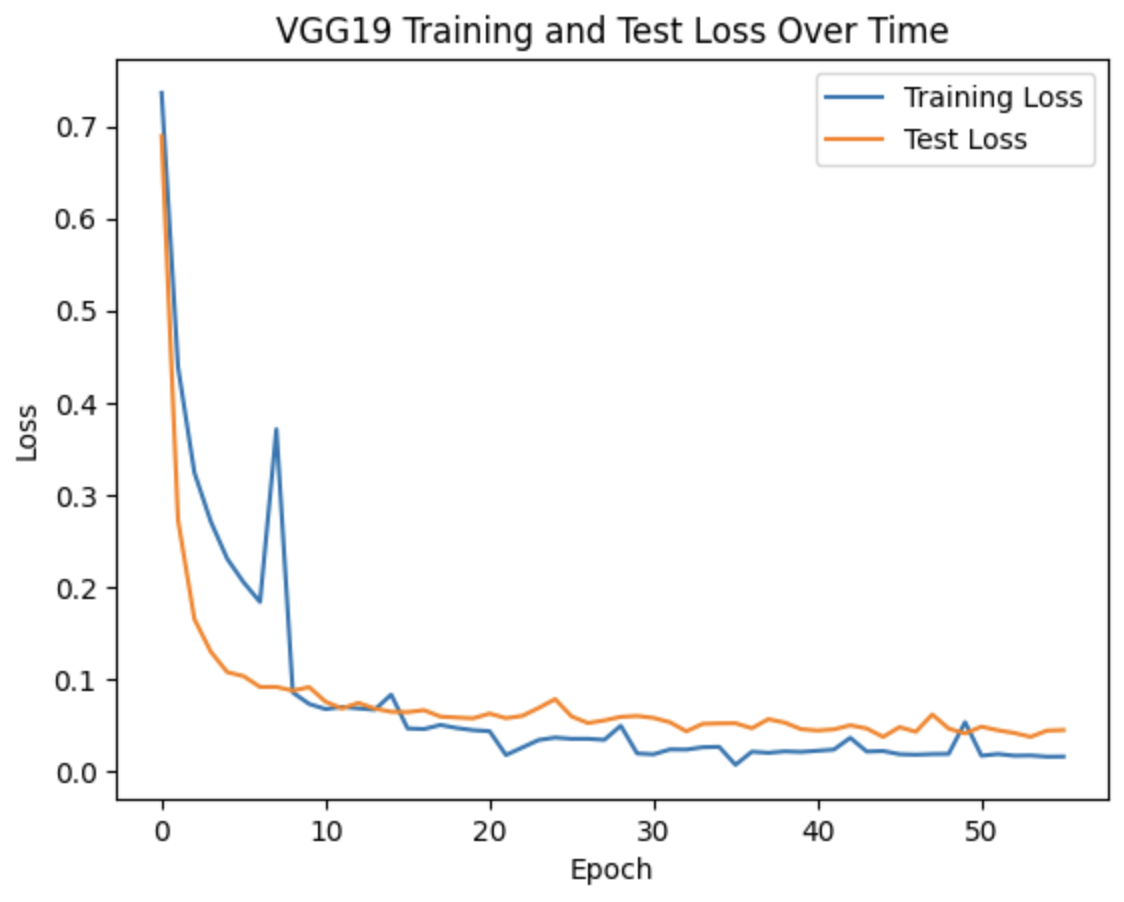
\includegraphics[width=\textwidth]{images/vggloss.png}
\end{minipage} \begin{minipage}{8cm}
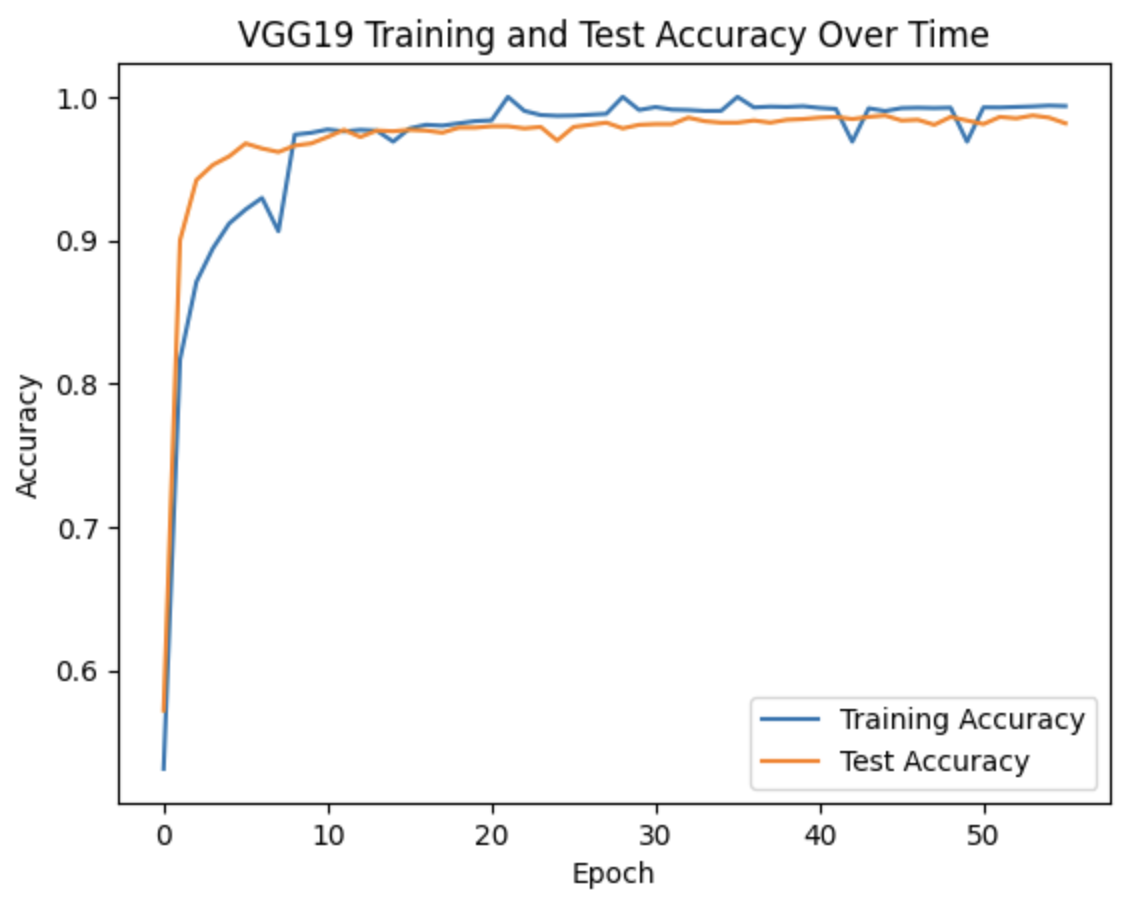
\includegraphics[width=\textwidth]{images/vggacc.png}
\end{minipage}
\caption{VGG19 fine-tuning training/testing loss, and training/testing accuracy}
\label{fig:vgg19training}
\end{figure}

\begin{figure}[H]
\centering
\begin{minipage}{8cm}
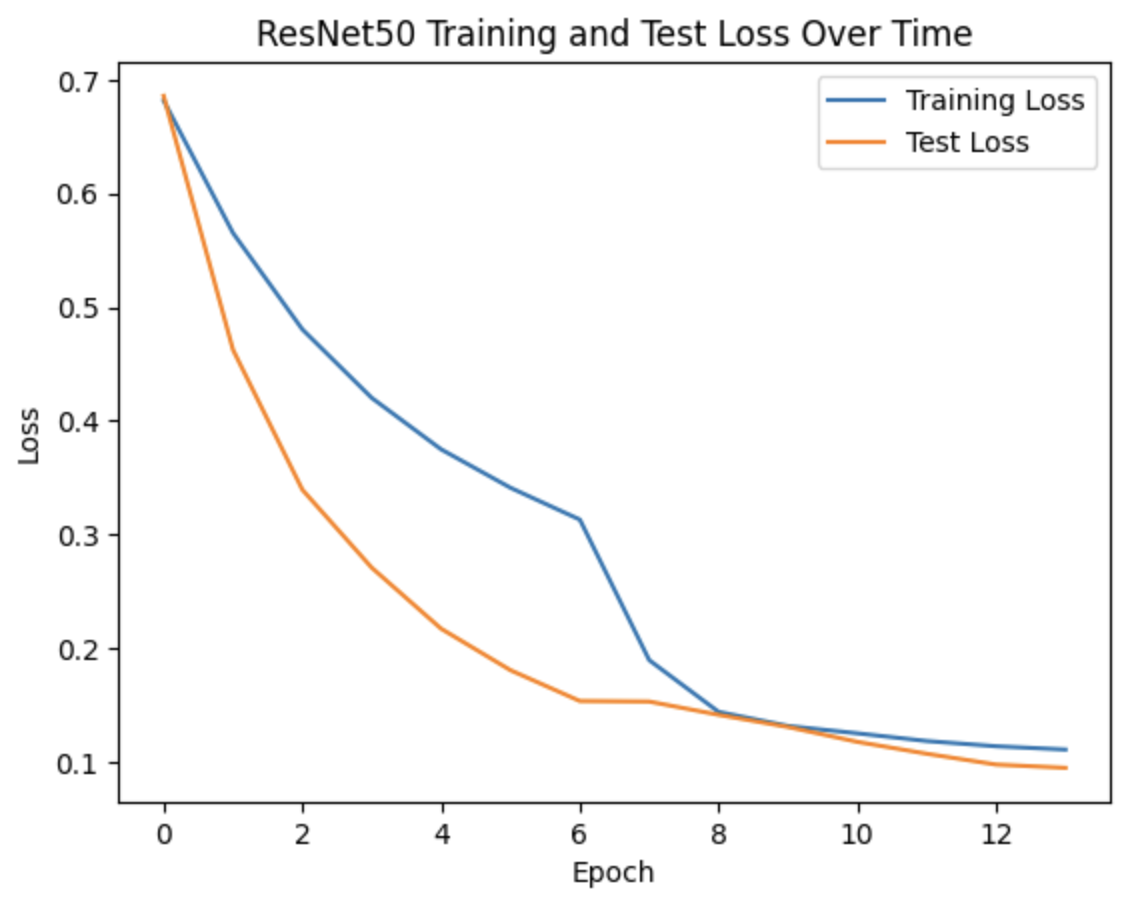
\includegraphics[width=\textwidth]{images/resnetloss.png}
\end{minipage} \begin{minipage}{8cm}
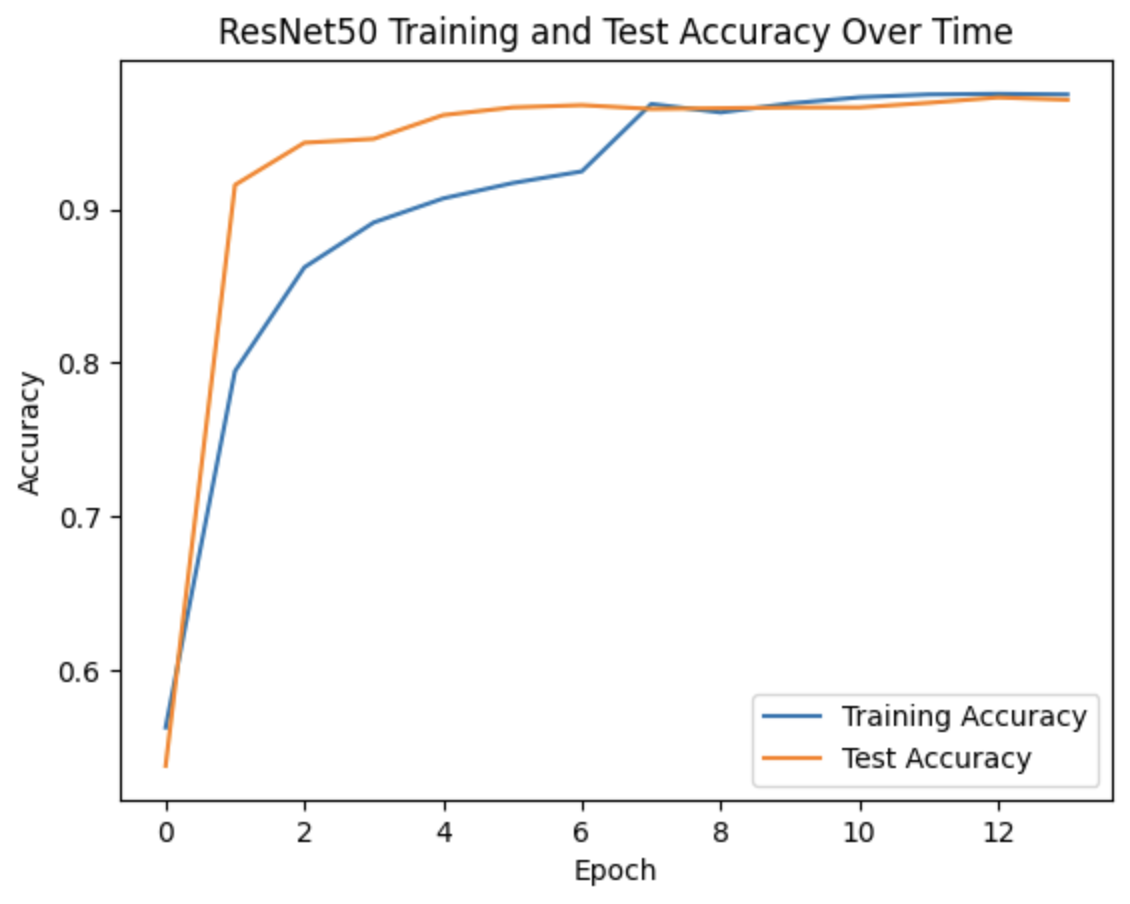
\includegraphics[width=\textwidth]{images/resnetacc.png}
\end{minipage}
\caption{ResNet50 fine-tuning training/testing loss, and training/testing accuracy}
\label{fig:resnet50training}
\end{figure}

\section{Diffusion training details}\label{sec:diffusionAppendix}

The procedure for turning any diffusion model into a classifier, as described in \cite{liYourDiffusionModel}, is as follows. Normal class-conditional diffusion models are trained to optimize the ELBO objective, given by 
\[\mathcal{L}(c_i) = -\EE_{t,e}[\lVert\varepsilon - \varepsilon_{\theta}(x_t,c_i)\rVert^2],\]
where $\varepsilon$ is the true backwards noise at timestep $t$, given image $x_t$ and class $c_i$. In order to predict the class given an image, we want 
\[p_{\theta}(c_i|x) = \frac{p(c_i)p_{\theta}(x|c_i)}{\sum_j p(c_j)p_{\theta}(x|c_j)}.\]
Since the loss (i.e., approximately the ELBO) is the log likelihood of the probability of any given input, we can approximate 
\[p_{\theta}(c_i|x) \approx \frac{\exp\left(\mathcal{L}(c_i)\right)}{\sum_j \exp\left(\mathcal{L}(c_j)\right)}.\]
Each $\mathcal{L}(c_i)$ can be approximated with a Monte Carlo sampling from $(t_i, \varepsilon_i)$ to approximate the expected value, thus giving us a classifier.

With this method, we found training and inference to be a large bottleneck. For inference, accurate Monte Carlo estimates requires the number of samples to be on the order of thousands before results are not nonsensical. Each image prediction took our network roughly $3$ minutes on the smaller image size ($32$x$32$), with $1000$ samples per image. When we originally attempted to implement this method with larger image sizes ($256$x$256$), as with the other methods, training was on the order of an hour per epoch. After training the larger classifier for around $20$ hours, we realized that any attempt to optimize or interpret the model would not be realistic. 

We attempted to implement the classifier with a number of different architectures, including UNets with and without self attention, $T$ timesteps equal to $1000$ and $4000$, and with linear and cosine scheduling. Out of all of these combinations, we found that $T=4000$, cosine scheduling, and self attention produced the best results. Since we were restricted to $32$x$32$ images due to the time and compute required to train a full model, our classification results were technically not a fair comparison with the deep CNN classifier results. 

\section{Style-content reconstruction}\label{sec:stylecontentreconstruction}

\begin{figure}[H]
  \centering
  % First row of images
  \begin{subfigure}[b]{0.3\textwidth}
  \centering
    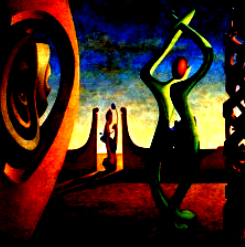
\includegraphics[width=3.5cm]{images/2_reconstructed_layer_0.png}
    \caption{VGG\_2\_class conv1\_1}
    \label{fig:image1}
  \end{subfigure}
  \hfill
  \begin{subfigure}[b]{0.3\textwidth}
  \centering
    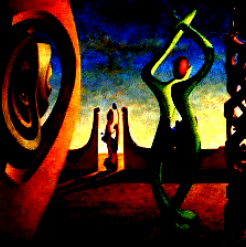
\includegraphics[width=3.5cm]{images/2_reconstructed_layer_5.png}
    \caption{VGG\_2\_class conv2\_1}
    \label{fig:image2}
  \end{subfigure}
  \hfill
  \begin{subfigure}[b]{0.3\textwidth}
  \centering
    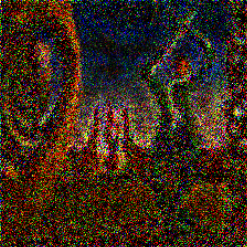
\includegraphics[width=3.5cm]{images/2_reconstructed_layer_10.png}
    \caption{VGG\_2\_class conv3\_1}
    \label{fig:image3}
  \end{subfigure}

  % Second row of images
  \begin{subfigure}[b]{0.3\textwidth}
  \centering
    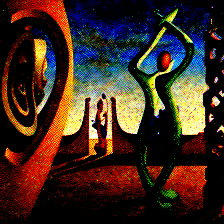
\includegraphics[width=3.5cm]{images/reconstructed_layer_0.png}
    \caption{VGG\_10\_class conv1\_1}
    \label{fig:image4}
  \end{subfigure}
  \hfill
  \begin{subfigure}[b]{0.3\textwidth}
  \centering
    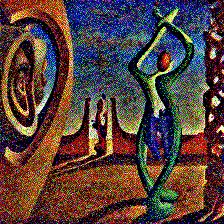
\includegraphics[width=3.5cm]{images/reconstructed_layer_5.png}
    \caption{VGG\_10\_class conv2\_1}
    \label{fig:image5}
  \end{subfigure}
  \hfill
  \begin{subfigure}[b]{0.3\textwidth}
  \centering
    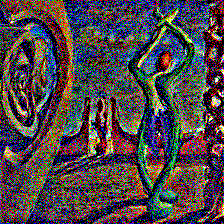
\includegraphics[width=3.5cm]{images/reconstructed_layer_10.png}
    \caption{VGG\_10\_class conv3\_1}
    \label{fig:image6}
  \end{subfigure}

  \caption{Top Row: content reconstructed from VGG\_2\_class. Bottom row: content reconstructed from VGG\_10\_class. Notably, the $2$ class reconstructions are sharper, since the network is more finetuned.}
  \label{fig:4.2_content_reconstruction}
\end{figure}

\section{Neural Style Transfer Trajectories}\label{sec:trajectories}

\begin{figure}[H]
    \hfill
    \begin{minipage}{0.75\textwidth}
    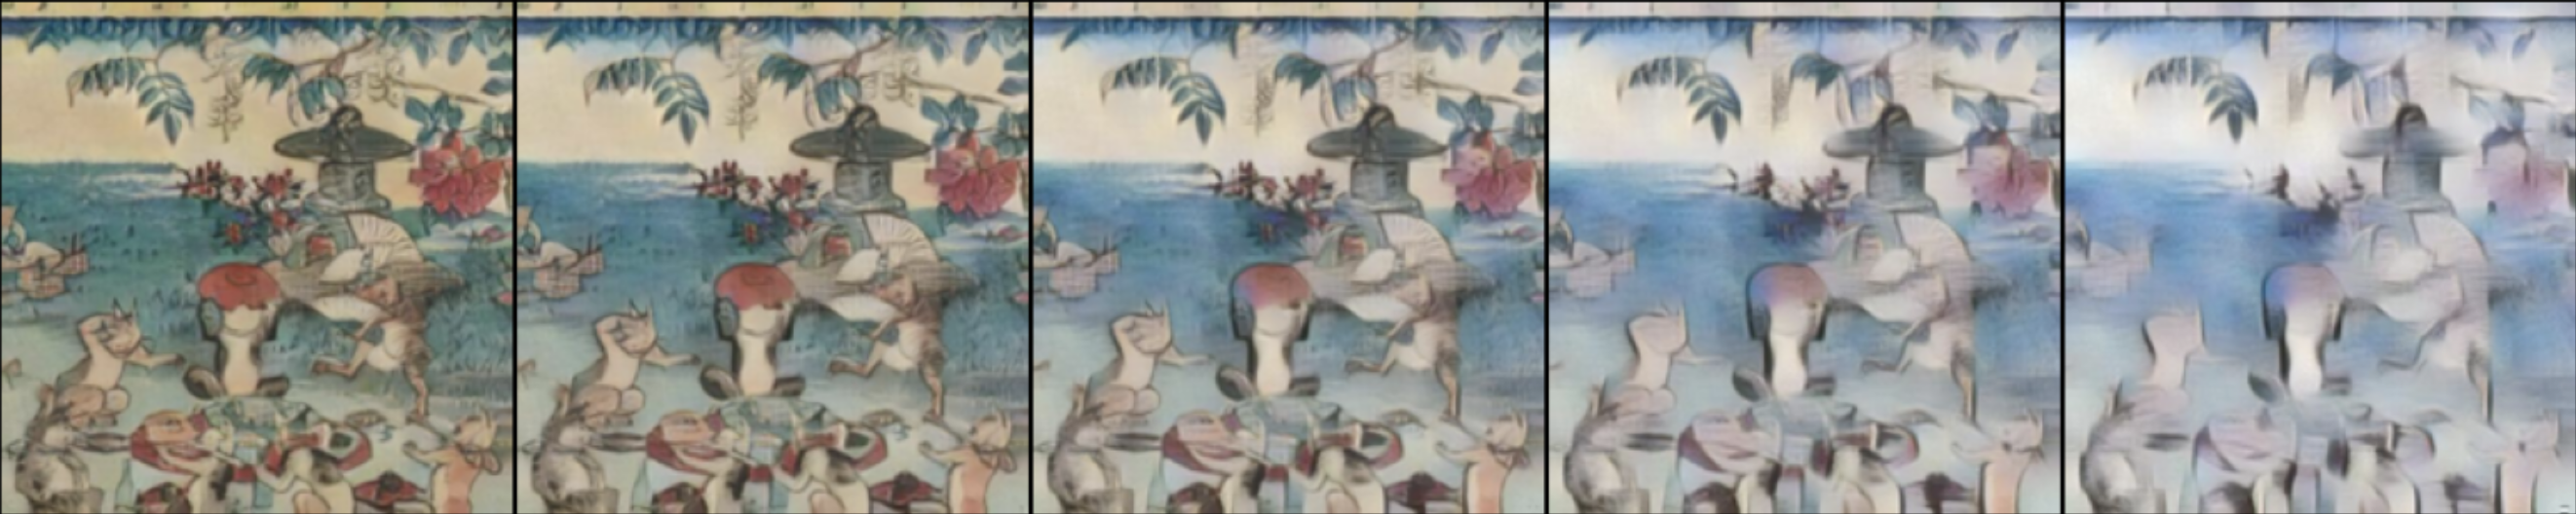
\includegraphics[width=\textwidth]{images/ukiyo_e.png}
    \end{minipage}
    \hfill
    \begin{minipage}{0.15\textwidth}
    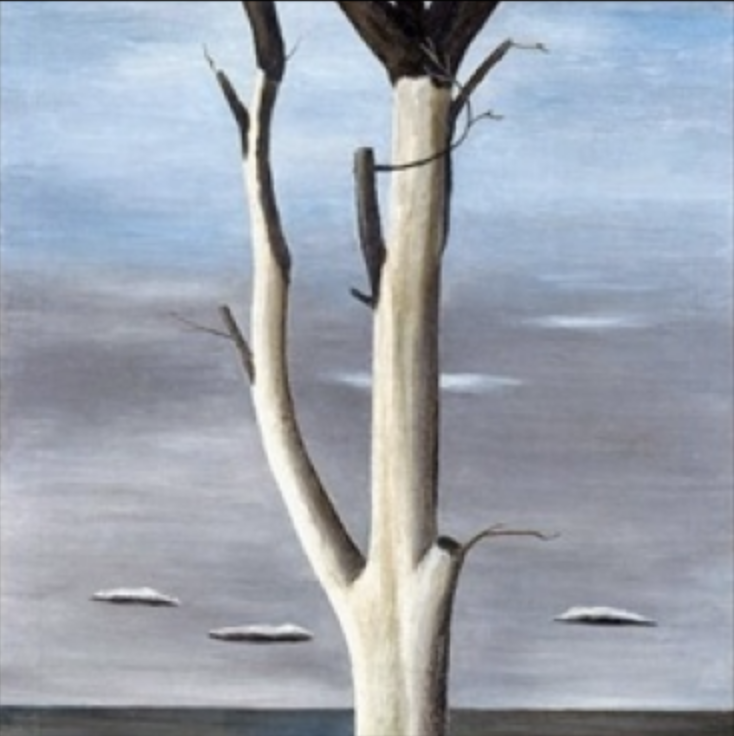
\includegraphics[width=\textwidth]{images/surrealist.png}
    \end{minipage}
    \hfill\hfill
    \caption{Arbitrary neural style transfer with a surrealist style image (very right), on a ukiyo\_e content image, with alpha values $\alpha=0,0.25,0.5,0.75,1$ from left to right. }
    \label{fig:nstex}
\end{figure}

\begin{figure}[H]
    \centering
    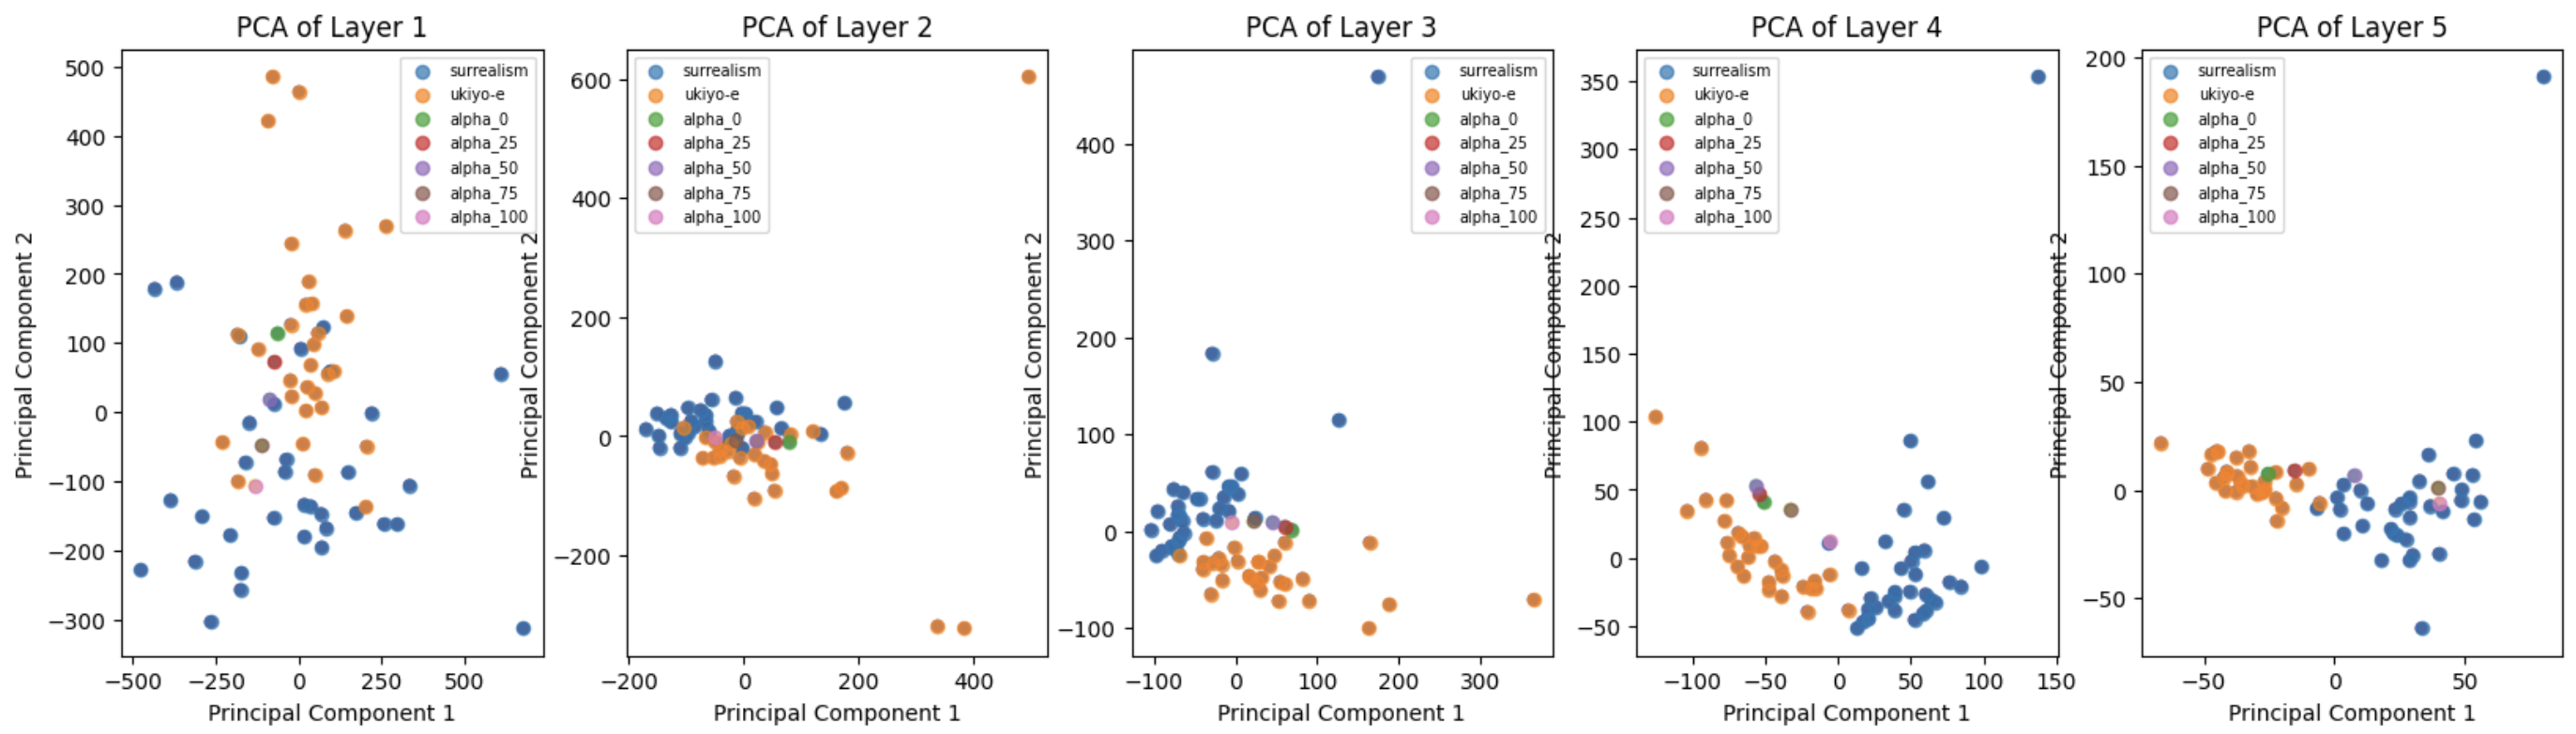
\includegraphics[width=18cm]{images/singletrajectory.png}
    \caption{PCA trajectory of the arbitrary neural style transfer depicted in Figure~\ref{fig:nstex}}
    \label{fig:pcatraj}
\end{figure}

It is noteworthy that the pattern observed in Section~\ref{sec:casestudy} becomes even more pronounced when we repeat this procedure with multiple images: 

\begin{figure}[H]
    \centering
    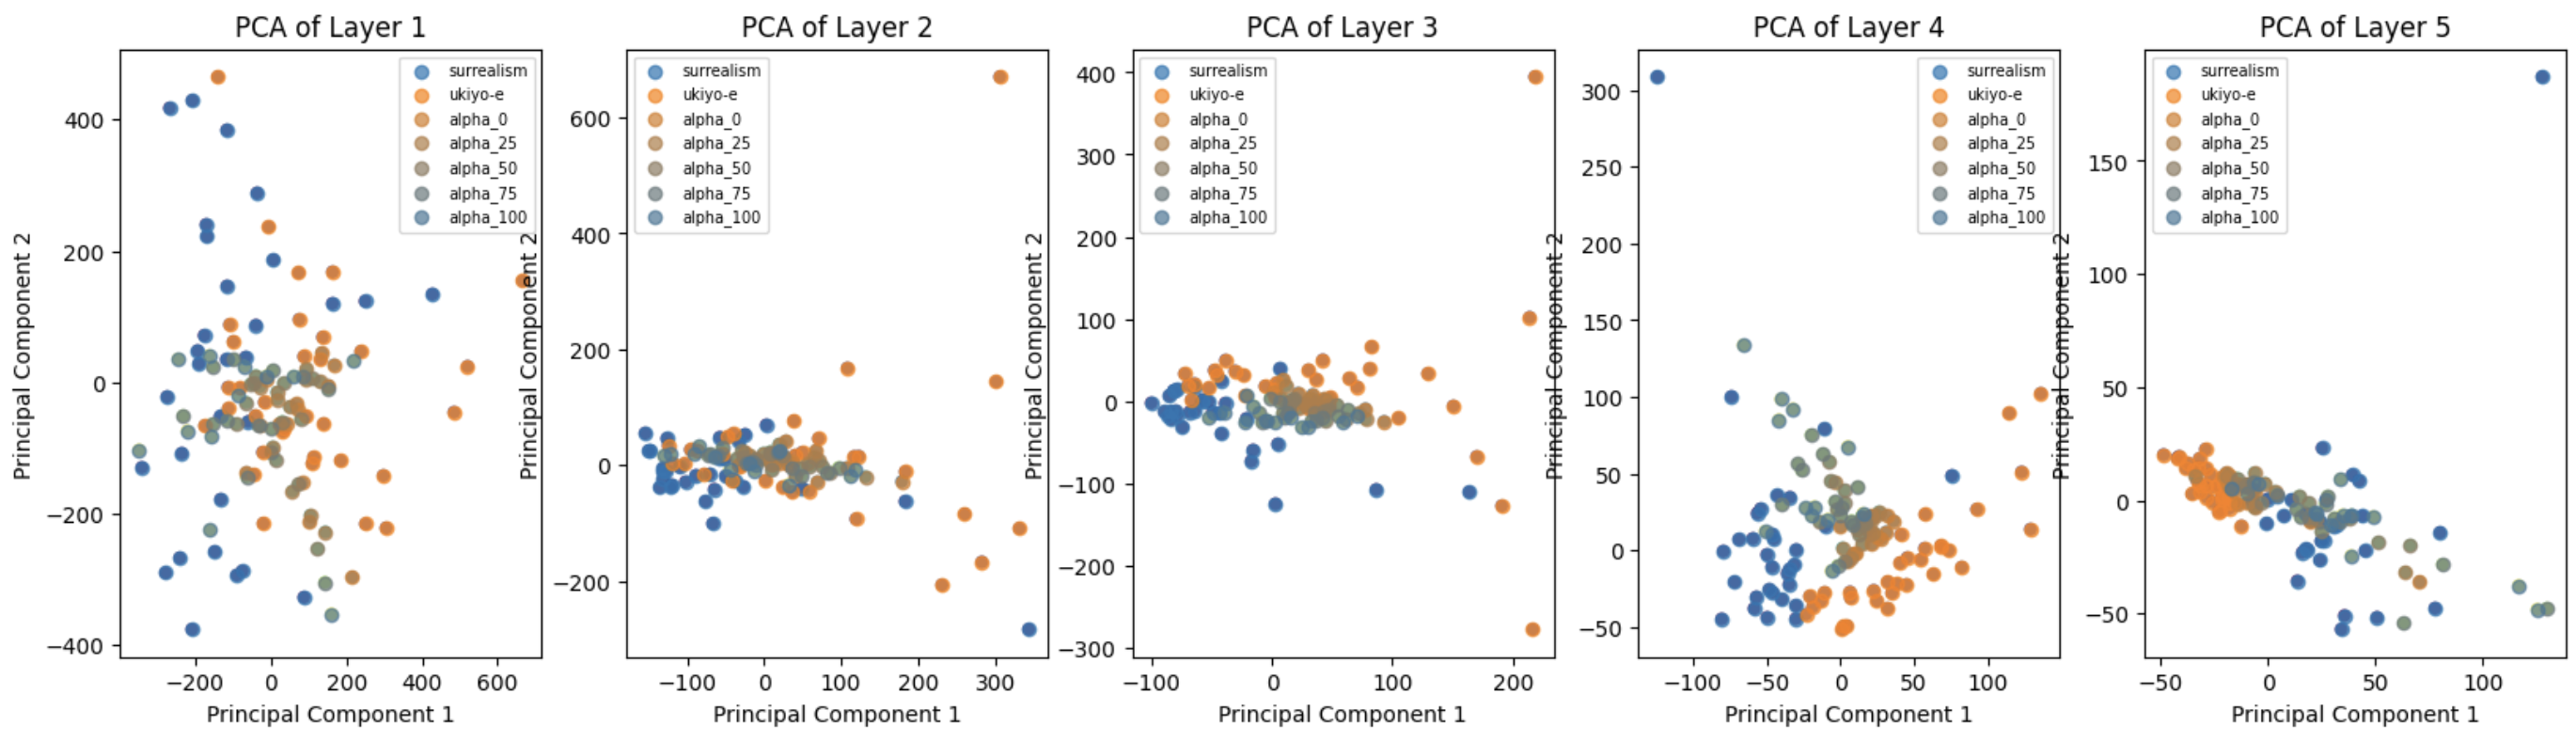
\includegraphics[width=18cm]{images/manytrajectories.png}
    \caption{PCA trajectories}
    \label{fig:pcatrajs}
\end{figure}

In Figure~\ref{fig:pcatrajs}, we repeat the procedure in Figures~\ref{fig:nstex} and~\ref{fig:pcatraj} for twelve (\verb|surrealist| style, \verb|ukiyo_e| content) image pairs, where each pair contributes five data points ($\alpha\in \{0,0.25,0.5,0.75,1\}$) to each of the five layers. The results are almost the same, but more pronounced, than the results in Section~\ref{sec:casestudy}. In particular, there is a lot of variance in the first layer, which agrees with our hypothesis that style representations are not yet reliable early in the network. However, by layer $4$, we observe a clear gradient from the orange \verb|ukiyo_e| images to the blue \verb|surrealism| images, with increasing $\alpha$ values creating linear layers. This suggests that this point in the network has very strong and reliable interpretations of style. 

\end{document}